%!TEX root = ../../main.tex


\begin{figure}[!htb]
\centering
%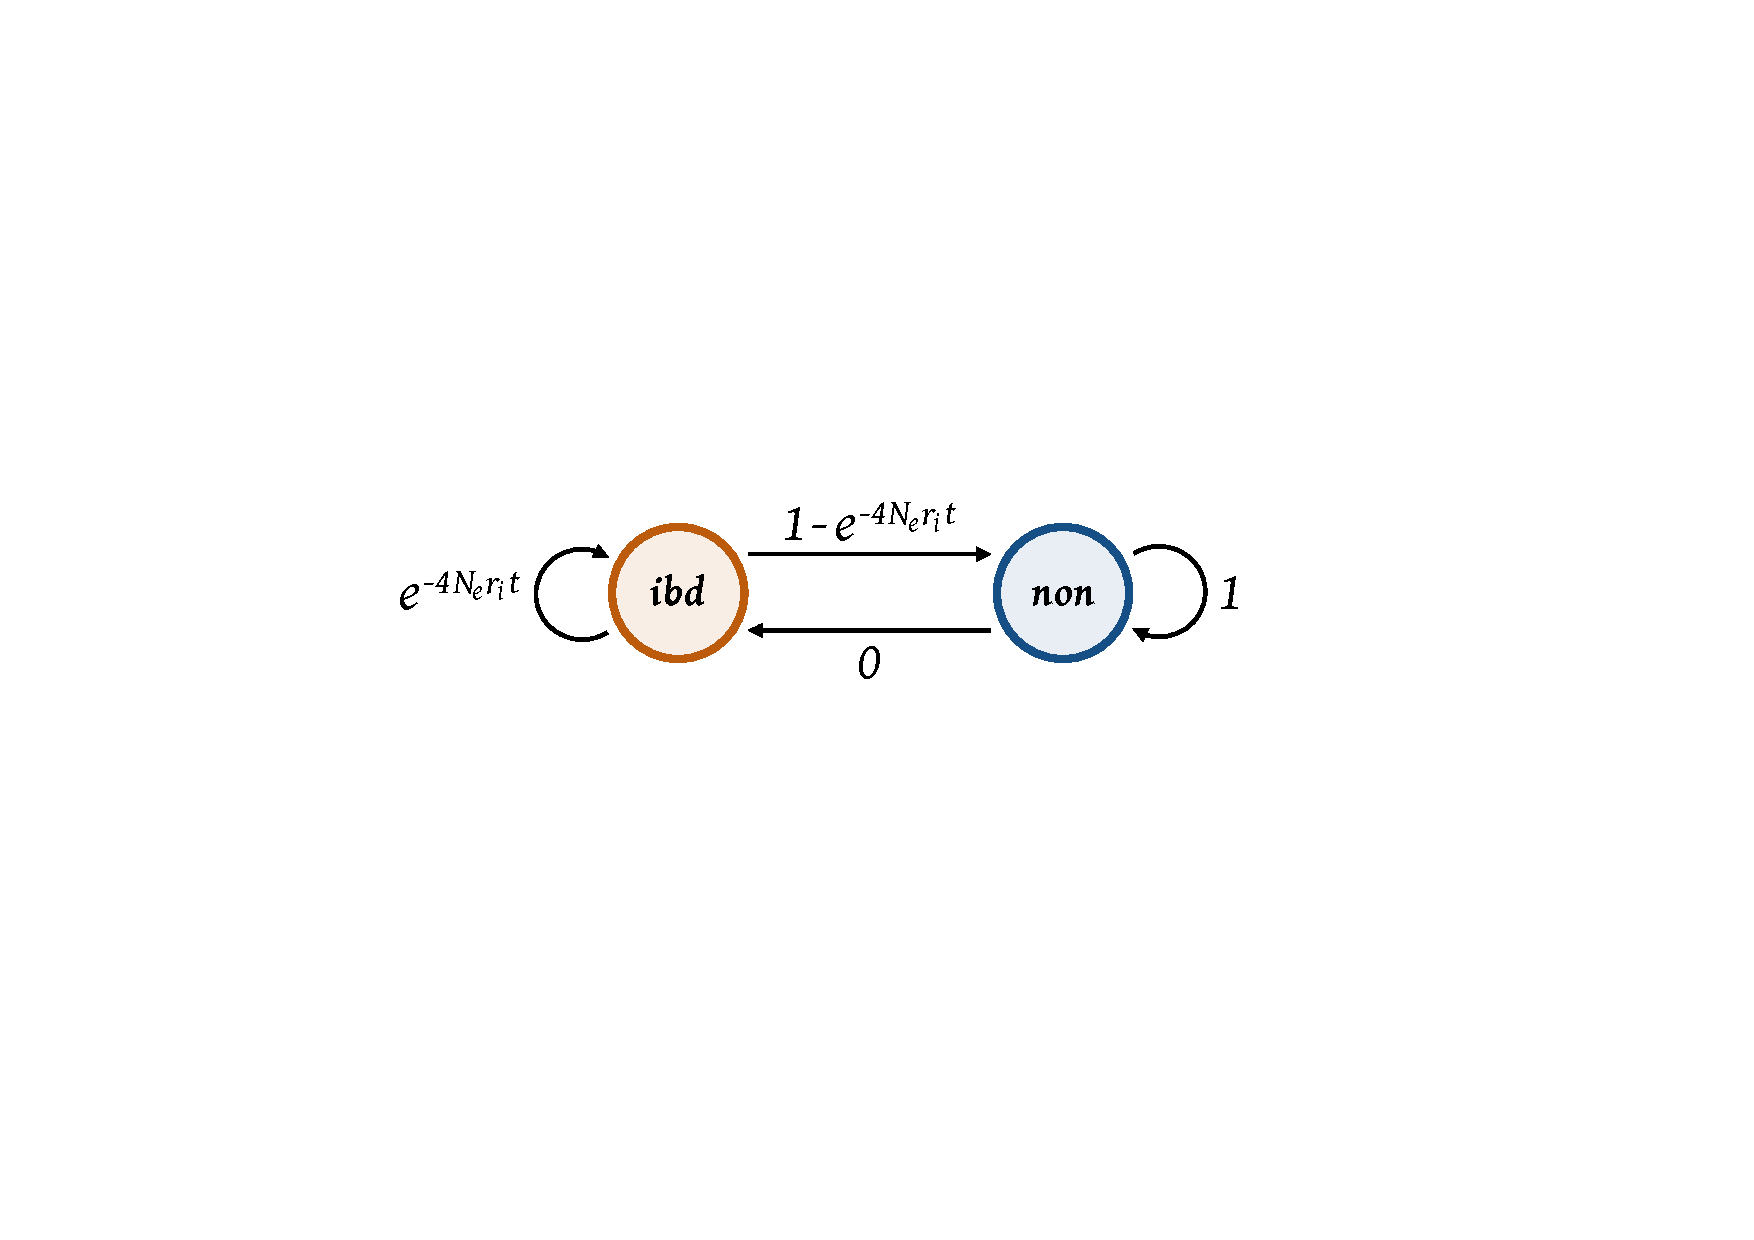
\includegraphics[width=0.75\textwidth]{./img/ch4/hmm_trans}\\

\vspace{5pt}
\begin{tikzpicture}[->,>=stealth,auto,thick,
txt/.style={font=\sffamily\small,text width=2.5cm},
sub/.style={circle,draw=white, fill=white,minimum size=1.75cm},
state/.style={circle,draw,ultra thick,minimum size=1.5cm,outer sep=2pt,font=\bfseries\Large},
dbl/.style={diamond,draw=black!50,thick,minimum size=1.45cm,outer sep=2pt},
obs/.style={diamond,draw=black,fill=white,fill opacity=0.5,text opacity=1,thick,minimum size=1.5cm,outer sep=2pt,font=\bfseries}]

\newcommand{\observeIBD}[4]{
\draw[->,draw=DarkOrange2!20,ultra thick] (#1) to (#2);
\draw[->,draw=DarkOrange3,densely dotted] (#1) -- (#2) node [pos=#4,anchor=center,fill=white,font=\small,inner sep=2pt] {#3};
}
\newcommand{\observeNON}[4]{
\draw[->,draw=DodgerBlue3!20,ultra thick] (#1) to (#2);
\draw[->,draw=DodgerBlue4,densely dotted] (#1) -- (#2) node [pos=#4,anchor=center,fill=white,font=\small,inner sep=2pt] {#3};
}

\node[txt] at (-1, 4) {Hidden\\states, $S$};
\node[txt] at (-1, 0) {Observation\\states, $H$};

\node[sub] (I) at (3.5,4) {};
\node[sub] (N) at (8.5,4) {};

\node[state,draw=DarkOrange3,fill=DarkOrange1!25] (ibd) at (3.5,4) {\emph{ibd}};
\node[state,draw=DodgerBlue4,fill=DodgerBlue1!25] (non) at (8.5,4) {\emph{non}};

% \node[dbl] (s00) at (1,0.84) {};
% \node[dbl] (s01) at (3,0.84) {};
% \node[dbl] (s02) at (5,0.84) {};
% \node[dbl] (s11) at (7,0.84) {};
% \node[dbl] (s12) at (9,0.84) {};
% \node[dbl] (s22) at (11,0.84) {};

\node[obs] (h00) at (2,0)  {$h_{00}$};
\node[obs] (h01) at (6,0)  {$h_{01}$};
\node[obs] (h11) at (10,0) {$h_{11}$};

% \path (ibd.25)  edge node[above]{\Large{${1 - e^{-4 \Ne r_i \tau_k}}$}} (non.155);
\path (ibd.25)  edge node[above]{\large{$\varphi$}} (non.155);
\path (non.205) edge node[below]{\large{$0$}} (ibd.335);

% \path (ibd) edge [out=205,in=155,looseness=5] node[left] {\Large{${e^{-4 \Ne r_i \tau_k}}$}} (ibd);
\path (ibd) edge [out=205,in=155,looseness=5] node[left] {\large{$1-\varphi$}} (ibd);
\path (non) edge [out=25,in=335,looseness=5] node[right] {\large{$1$}} (non);

% \observeIBD{I.315}{g22}{$\delta_{22}$}{0.25}
% \observeIBD{I.300}{g12}{$\delta_{12}$}{0.31}
% \observeIBD{I.285}{g11}{$\delta_{11}$}{0.4}
\observeIBD{I.300}{h11}{$\delta_{11}$}{0.2}
\observeIBD{I.280}{h01}{$\delta_{01}$}{0.35}
\observeIBD{I.260}{h00}{$\delta_{00}$}{0.5}

\observeNON{N.240}{h00}{$\eta_{00}$}{0.2}
\observeNON{N.260}{h01}{$\eta_{01}$}{0.35}
\observeNON{N.280}{h11}{$\eta_{11}$}{0.5}
% \observeNON{N.270}{g11}{$\eta_{11}$}{0.5}
% \observeNON{N.285}{g12}{$\eta_{12}$}{0.45}
% \observeNON{N.300}{g22}{$\eta_{22}$}{0.45}

\end{tikzpicture}
% \vspace{10pt}
%
% X
%
% \vspace{10pt}
% \begin{tikzpicture}[auto,thick,decoration={coil},
% line/.style={->,>=latex},
% rec/.style={->,>=stealth,rounded corners=4pt},
% txt/.style={font=\sffamily\small,text width=2.5cm},
% dna/.style={decorate,thick,decoration={aspect=0, segment length=0.5cm}},
% var/.style={rectangle,draw=black!50,fill=black!10,minimum size=0.4cm,outer sep=2mm,inner sep=2pt,font=\tiny\sffamily\bfseries}]
%
% \node[txt] at (-1, 5) {Genome};
% \node[txt] at (-1, 3.5) {Sample variant sequence};
%
% % \node[var] at (2.1,0) {};
% % \node[var] at (3.5,0) {};
%
% \foreach \v [remember=\v as \last (initially 1), count=\i] in {1.94,2.87,4.05,4.71,5.86,7.37,8.63,9.66,10.38}{
% 	\fill[gray!50] (\v - 0.05,4.6) rectangle (\v + 0.05,5.4);
% 	\coordinate (beg) at (\v,4.4);
% 	\node[var]  (end) at (\v,3.4) {\i};
% 	\draw[line] (beg) to (end.north);
% }
%
% \draw[dna, decoration={amplitude=.15cm}] (1.1,5) -- (11.5,5);
% \draw[dna, decoration={amplitude=-.15cm}] (1,5) -- (11.5,5);
%
% \fill[white] (0.9,4.6) rectangle (1.13,5.4);
% \fill[white] (11.2,4.6) rectangle (11.6,5.4);
%
% % \node[site] (1) at (1.0,2) {};
% %
% % \foreach \s [remember=\s as \last (initially 1)] in {2,...,10}{
% %   \node[site] (site\s) at (\s,2) {};
% %   \draw[line] (\last,2) to (site\s.west);
% % 	\node[site] (\s) at (\s,2) {};
% % }
%
% \end{tikzpicture}

\vspace{5pt}

\Caption{Illustration of the Hidden Markov Model for IBD inference}%
{\N{2} hidden states are assumed to generate the observations in a Markov process; \emph{ibd} and \emph{non}.
Transitions from each state into any state are indicated by \emph{solid} lines.
The probability of transition from \emph{ibd} to \emph{non} is denoted by $\varphi$, and from \emph{non} to \emph{ibd} is set to zero; hence, once the Markov chain proceeds into the \emph{non} state it cannot transition back into \emph{ibd}.
This is because the IBD process is modelled such that only the innermost IBD segment is inferred, relative to the focal position which sits at the start of the sequence.
The input sequence consists of genotype data from a pair of individuals, resulting in \n{6} possible observation states; denoted by $g_{k_1 k_2}$, where ${k_1,k_2 \in \lbrace 0,1,2 \rbrace}$.
The probabilities of emitting each possible genotype pair given each hidden state are denoted by $\delta_{k_1 k_2}$ and $\delta_{k_1 k_2}$ for \emph{ibd} and \emph{non}, respectively; indicated by the \emph{dotted} lines.
The direction of arrows indicates conditional dependence; \ie the transition from one hidden state into another state, or emission of a genotype pair while being in \emph{ibd} or \emph{non}.}%
{fig:info_hmm}
\end{figure}
